% 2011 年陕西卷理科第 17 题：圆 x^2+y^2=25 上的点 P，投影 D，PD 上的点 M 且 |MD|=4/5|PD|。
% 来源 PDF：普通高考/2011/2011陕西理.pdf，SHA-256 04dab6de0e3ee6223a1cbc126f7f83ae354d2b31201a14db1f31c8477d8a3bed。
% 原页：第 2 页第 1 栏上部，书页码 694。示意。
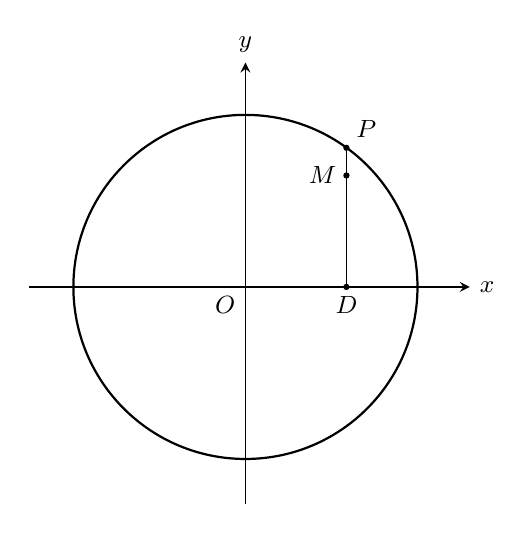
\begin{tikzpicture}[>=stealth, semithick, font=\small, scale=0.95]
  \draw[->] (-2.9,0)--(3.0,0) node[right] {$x$};
  \draw[->] (0,-2.9)--(0,3.0) node[above] {$y$};
  \draw[thick] (0,0) circle (2.3);
  \coordinate (P) at (1.35,1.86);
  \coordinate (D) at (1.35,0);
  \coordinate (M) at (1.35,1.49);
  \draw (P)--(D);
  \fill (P) circle (1.2pt) node[above right] {$P$};
  \fill (M) circle (1.2pt) node[left] {$M$};
  \fill (D) circle (1.2pt) node[below] {$D$};
  \node[below left] at (0,0) {$O$};
\end{tikzpicture}
